\chapter{The Baltic Sea}
\label{kap-einleitung}

In addition to the model investigations of tidal straining and sediment 
transport in the previous chapters, also several field campaigns were 
performed, focusing on the mechanisms of sediment transport in a non-tidal 
basin. These measurements were carried out in 
coastal areas of the Western Baltic Sea. Prior to the 
discussion of the data in the next chapter, an overview of the present 
hydrological conditions and the wave climate of the Baltic Sea is provided in 
the following. Additionally, the sedimentology of the 
Western Baltic Sea are briefly discussed, as the following chapter focuses on 
near-bottom dynamics and sediment transport.

% \section{History}
% 
% The Baltic Sea emerged from a subglacial lake at the end of the Weichselian Ice 
% Age, approximately 12,000 BP, and has since gone through several stages of 
% salty and brackish sea states or fresh water conditions, depending on whether a 
% connection to the open ocean was established or not. Indicators for this 
% alternations are, amongst others, changes in the benthic communities, and so the 
% nomenclature of the evolution stages was often determined by the prevailing 
% species.
% 
% With the retreat of the glaciers at the end of the Weichselian Ice Age, a 
% subglacial lake, together with water from the rapidly melting glaciers, formed 
% the \textit{Baltic Ice Lake}. Land uplift, that followed the deglaciation, 
% formed a landbridge between Sweden and the main land 11,200 BP, damming the 
% Baltic Ice Lake. Sea level was raised by glacial melt water until the lake began 
% to drain over the Öresund sill. Presumably, a lowering of the water level by 25 
% to 28 m by drainage through a channel near Mt. Billingen in central Sweden 
% happened very rapidly around 10,300 BP, when the retreating ice margin collapsed 
% \citep[][]{bjoerk95,tikkanen2002} and a connection to the sea was opened. 
% 
% This new stage of the Baltic with a lower sea level is known as \textit{Yoldia 
% Sea} (from the marine mollusc \textit{Portlandia (Yolida) arctica} 
% \citep[][]{schoning2001}). There are no indicators for salt water entrainment 
% into the Yoldia Sea until global sea level rise and deglaciation formed a 
% connection through the Närke Strait 300 years later \citep[][]{schoning2001}. 
% This lead to brackish water conditions followed by decreasing salinity after the 
% straits had become too narrow to allow water exchange another 100 to 300 years 
% later \citep[][]{bjoerk95}.
% 
% After the glaciers retreated, uplift of the land was not be compensated by 
% global sea level rise. Connection to the ocean was closed again around 9,500 BP, 
% and the regime shifted to fresh water conditions again, now called 
% \textit{Ancylus Lake} (after the freshwater gastropod \textit{Ancylus 
% fluviatilis} \citep[][]{tikkanen2002}). Although narrow outlets existed, the 
% surface of the Ancylus Lake rose up to 10 m above global sea level, inundating 
% extensive areas of land. This phase, called the Ancylus Transgression, ended 
% around 9,200 BP, when the sea level height exceeded the height of the Darss Sill 
% and water began to flow out through an evolving river system in the land 
% connection between Sweden and Germany \citep[][]{tikkanen2002}. Around 9,000 BP 
% this so-called Ancylus Regression ended when the water level reached global sea 
% level. The connection to the ocean through the river system remained, but no 
% extensive saline intrusion happened for the next 1,000 years.
% 
% Ongoing global sea level rise deepened the connection between the Baltic Basin 
% and the open ocean, letting more and more saline water enter the Ancylus Lake. A 
% short transition stage called \textit{Mastogloia Sea} (\textit{Mastogloia} are 
% diatoms that live in slightly saline conditions \citep[][]{eronen2001}) was 
% followed by the \textit{Litorina Sea} (named after the brackish water gastropod 
% \textit{Littorina littorea} \citep[][]{eronen2001}), when a great extent of 
% saline water entered the Baltic basin through the Straits of Denmark in 7,500 BP 
% \citep[][]{bjoerk95}. Transgression took place until the rise in ocean levels 
% ended 6,000 to 5,000 BP. When the Straits of Denmark became shallower, as land 
% uplift continued, water exchange was reduced and salinity in the Litorina Sea 
% declined down to the present brackish state in 4,000 BP, at first named 
% \textit{Limnea Sea} (from the snail \textit{Lymnaea ovata}), and finally, since 
% 500 BP, \textit{Mya Sea} (after the Northern American clam \textit{Mya 
% arenaria}, which was brought into the Baltic by Viking ships 
% \citep[][]{bjoerck2008}).
% 

% 
 \section{Present hydrography and dynamics}
 
 \begin{figure}[ht]
  \flushleft
  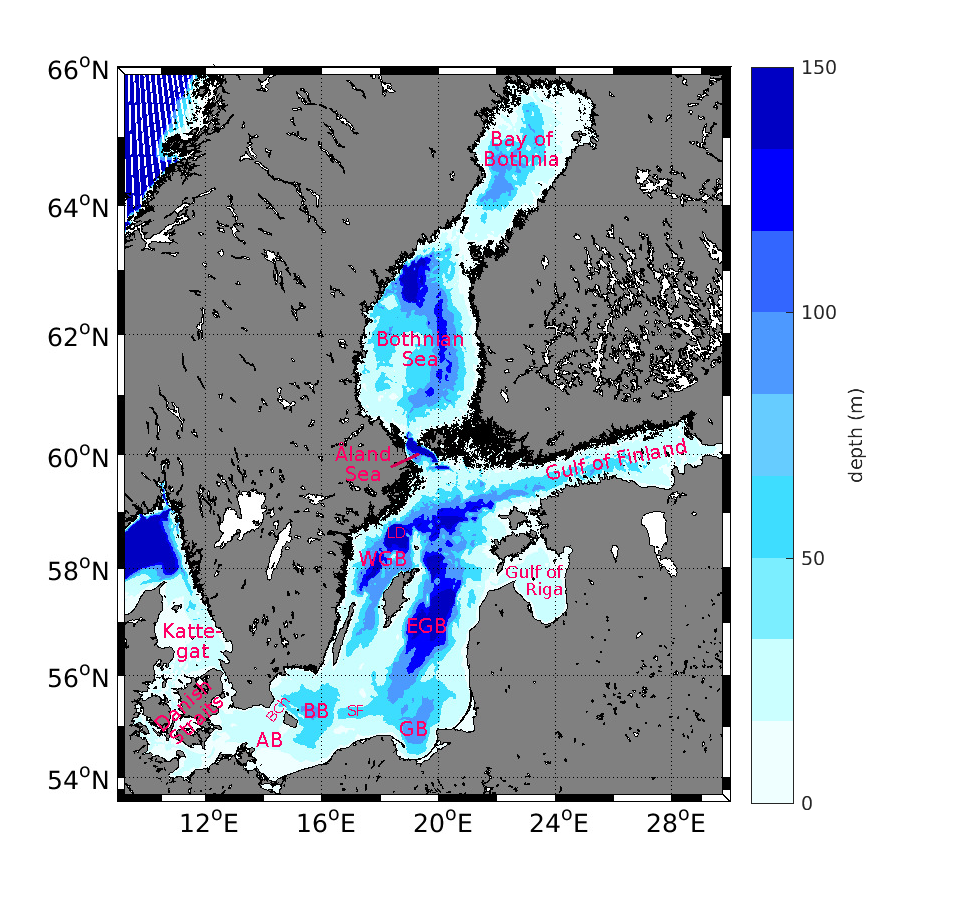
\includegraphics[width=17cm]{bilder/baltic.pdf}
  \caption{Topographic map of the Baltic Sea. Abbreviations stand for Arkona 
 Basin (AB), Bornholm Channel (BCh), Bornholm Basin (BB), S\l upsk Furrow (SF), 
 Gda\`{n}sk Basin (GB), Eastern Gotland Basin (EGB), Landsort Deep (LD) and 
 Western Gotland Basin (WGB).}\label{balticmap}
 \end{figure}
 
The Baltic Sea has an extent of $4.2 \times 10^{5} \, \text{km}^2$ 
\citep[][]{balticsea} and is connected to the North Sea via the Danish Straits: 
the \O resund and the Great and Little Belt together with the Fehmarn Belt. The 
climate is humid: Annual precipitation adds around 224 $\text{km}^3$ of water to 
the Baltic Sea, evaporation amounts to only 184 $\text{km}^3$. Rivers discharge 
a total of 436 $\text{km}^3$ water per year \citep[][]{reissmann2009}. An 
exchange flow takes place, where brackish water leaves the Baltic Sea near the 
surface (annually around 947 $\text{km}^3$) and saline North Sea water enters at 
the bottom (nearly 500 $\text{km}^3$ per year on average, but frequency and 
strength of inflow events differ dramatically over time, highly dependent on 
short-term weather conditions). The saline and oxic waters intruding from the 
North Sea are the only 
source of oxygen for the deeper parts of the Baltic Sea. Inflows occur in two 
different ways. Baroclinic inflows are triggered by the horizontal salinity 
gradient between North and Baltic Sea and occur at calm wind conditions, mostly 
in summer \citep[][]{reissmann2009}. The main contribution to the ventilation 
of the 
deep basins is, however, provided by the barotropic inflow events, called Major 
Baltic Inflows (MBIs). Those MBIs occur irregularly and are caused by special 
meteorological conditions: Firstly, high air pressure over the Baltic Sea 
region and strong winds in westerly directions cause the mean sea level in the 
Baltic Sea to drop by up to 50 cm, imposing a gradient in sea level elevation 
between the Kattegat and the Arkona Basin. Secondly, several weeks of wind in 
easterly 
directions with strong gales \citep[][]{balticsea, reissmann2009, mohrholz2015} 
push saline and oxygen rich water into the Baltic Sea. These conditions occur 
primarily between October and February. 
% Since records 
% started in 1897, MBIs were on a rather regular base up to the 1970s. After 
% this, 
% long periods without inflow events decreased oxygen supply in the Baltic basins 
% drastically. The last MBIs were in 1993 and 2003, but they interrupted the 
% anoxic conditions in the deep water only for short periods of time 
% \citep[][]{schinke1998, mohrholz2015}. 

Two shallow sills, the Dr\o gden Sill (7 m deep, values in brackets refer to the 
local depth in the following) and the Darss Sill (18 m) form the passage to the 
first of several basins, the Arkona Basin (45 m), 
through which the North Sea water propagates as a deep gravity current 
(see \fig{balticmap}). Through 
the Bornholm Channel, the Arkona Basin is connected to the Bornholm Basin (80 
m), from where the bottom current flows over the S\l upsk Sill (60 m) and 
through the approximately 80 km long S\l upsk Furrow (90 m) southeast into the 
Gda\`{n}sk Basin (110 m) and northeast into the Eastern Gotland Basin (250 m). 
From there, the deep current can enter the easterly Gulf of Riga or the Western 
Gotland Basin, wherein the Landsort Deep (with 490 m the deepest point in the 
Baltic Sea) is located. The Gulf of Finnland forms the eastern boundary of the 
Baltic Sea and north of the Gotland Basin, the \r{A}land Sea separates the 
Baltic Proper in the south from the Bothnian Sea and the Bay of Bothnia in the 
north \citep[][]{reissmann2009}. Salt water entering at the Darss Sill needs 
approximately 2--6 months to exchange the bottom water in the Gotland Basin 
\citep[][]{balticsea}.

The bathymetry of the Baltic Basin and the narrow connection to the 
open ocean via the Danish Straits lead to several notable features in the 
hydrographic conditions: Dense bottom water from the North Sea 
creates a permanent strong halocline that separates bottom from surface waters, 
preventing the ventilation of the water masses in the deep basins. Oxygen that 
enters through exchange with the atmosphere is not mixed below the halocline, 
leaving inflowing North Sea water as the only significant supply of oxygen. 
Large parts 
of the Baltic Sea become anoxic after long periods without large salt 
water inflows, with severe implications for the geochemical processes and the 
ecosystem of both the lower part of the water column and the sediment-water 
interface. 

Furthermore, a salinity gradient is present across the Baltic Sea: The bottom 
current entrains with overlying brackish water along its pathway (for 
example, volume of the gravity current increases by 53 \% when passing through 
the Arkona Basin, \citep[see][]{reissmann2009}), and the slow entrainment of 
salty water into the overlying water mass forms a NE--SW surface salinity 
gradient. Surface salinity drops from around 18~g~kg$^{-1}$ in the Danish 
Straits to 8~g~kg$^{-1}$ in the Arkona Basin, down to 6--7~g~kg$^{-1}$ in the 
Eastern Gotland Basin and even below 3~g~kg$^{-1}$ in the Bay of Bothnia and the 
Gulf of Finnland \citep[][]{balticsea}.

Besides the dense bottom currents originating from inflowing North Sea water, 
local wind forcing combined with the topographic structure and the permanent 
salinity stratification in the Baltic Sea triggers other flow features on 
smaller scales. Although tides do not play a significant role, other 
oscillatory currents are found in the Baltic Sea: near-inertial waves, internal 
seiching motions and topographic or coastal-trapped waves.
In the absence of tides and due to the permanent deep-water stratification, 
inertial oscillations and low-mode near-inertial wave motions have been found to 
dominate the energetics on the basin-scale \citep[][]{vanderlee2011}. 
Near-inertial internal waves have periods close to the inertial period, which is 
$T_f = 14.8$ h in the southern part of the Baltic Sea (at a latitude of 
$54^{\circ}$N) down to $T_f = 13.1$ h in the northern part ($66^{\circ}$N). 
Tide gauge records along the coast indicate that eigenoscillations play a 
major role in the Baltic Sea \citep[][]{wubber1979}. Large-scale meteorological 
forcing initiates the development of seiches on several frequencies, depending 
on which parts of the Baltic act as oscillatory system. 
 Another main energy source on basin-scale are topographic waves with periods 
of a few days, that are a direct response to enhanced wind forcing 
\citep[][]{holtermann2012}, and low-frequency, quasigeostrophic, 
coastal-trapped motions forced by local wind \citep[][]{pizarro1998}.

\section{Wave climate}\label{balticswan}

Another important factor for the dynamics in the Baltic Sea, especially 
in the context of sediment resuspension, are wind-generated waves. The impact 
of the wave-induced stress on the sediment generally dominates over the stress 
induced by the mean currents \citep[][]{Grant1986}, if the water is shallow 
enough to allow wave energy to reach the sea floor. To map the wave activity 
spatially resolved in the whole Baltic Sea, a wave model was set up, verified 
and model results were analyzed. This is described in the following.

\subsection{Wave model setup and verification}

The SWAN wave model version 41.01 was set up for the Baltic Sea including a 
nesting in the south-western part that was a focal point for the sediment 
transport investigations described in the following chapter. For the whole 
Baltic Sea, a grid 
resolution of $0.5^\circ \times 0.1^\circ $ in Latitude and Longitude was 
chosen 
in a domain reaching from $53.5^\circ \text{N } 9^\circ \text{E}$ to $66^\circ 
\text{N } 31^\circ \text{E}$. This includes the Kattegat, the passage from the 
Baltic to the North Sea, where boundary conditions were prescribed in the east: 
A constant JONSWAP spectrum with a wave height of $1$ m, a period of $5$ s and 
peak wave direction of $90^\circ$ with a high directional spreading. The 
passage 
from the North to the Baltic sea is very shallow, so the boundary conditions 
have negligible influence on the model outcome. Wave frequency range was set to 
0.1 to 1.8 Hz, which mirrors the actual wave frequencies occurring in the 
Baltic Sea \citep[][]{balticsea}, with a resolution of $42$ frequency bins. 
Computations included a spin-up time of $10$ days, sufficient for wave 
modeling, 
and were carried out for the years 2013 and 2014. The model was forced by wind 
data from the German Weather Service (DWD), the computational time step was $1$ 
hour (note that the propagation scheme implemented in SWAN is implicit, so the 
time step is not restricted by numerical issues). 

The nesting area reached from $53.5^\circ \text{N } 10^\circ \text{E}$ to 
$55.5^\circ \text{N } 15^\circ \text{E}$, including the Western German coastal 
seas. Spatial resolution was $0.01^\circ \times 0.025^\circ $ in Latitude and 
Longitude and the computational time step was set to $15$ minutes. Boundary 
conditions came from the Baltic Sea model and all parameters were left 
unchanged.

In \fig{verify} the significant wave height calculated with the wave model was 
compared to data obtained with a wave rider buoy. The significant wave height 
is defined as the average wave height of the highest one-third of the waves. 
This value matches the visually observed wave height best and can be calculated 
from the zeroth-order moment of the variance density spectrum $m_0$ via 
$H_s = 4 \sqrt{m_0}$ (see Appendix D for details).

\begin{figure}[ht]
 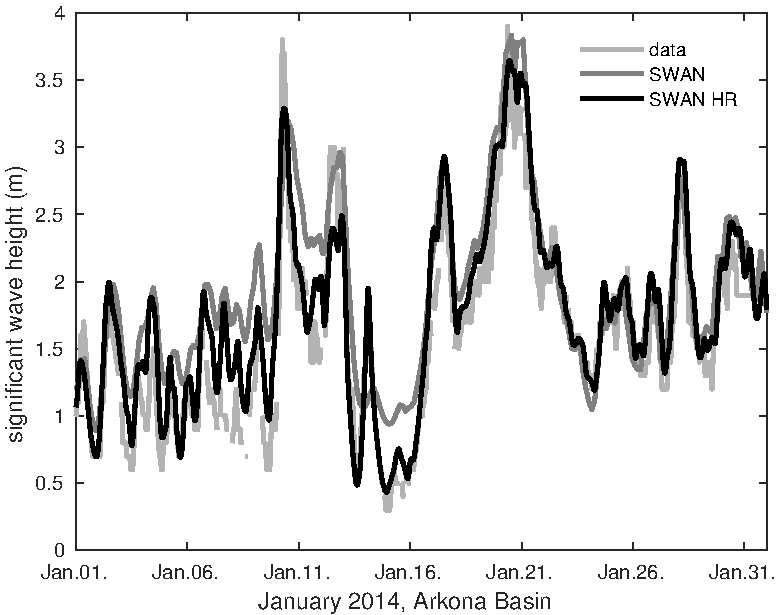
\includegraphics[width=15cm]{bilder/januar.pdf}
 \caption{Significant wave height calculated with the SWAN wave model (HR 
refers to the high resolved nested run) and measured wave height from the 
Arkona wave rider buoy.\label{verify}}
\end{figure}

In the context of a Master Thesis \citep[][]{masterarbeitronja}, the model 
setup for 2013 (still using the previous version SWAN 40.91AB) was 
extensively tested for numerical convergence and compared to measured data on 
several locations in the Baltic Sea. Wave parameters like significant wave 
height were in good agreement with available data, even in areas with complex 
topography. A brief description of wind wave properties and processes and a 
discussion the wave model SWAN can be found in Appendix D.

\subsection{Wave-Induced Bottom Friction Velocity Distribution}

Bottom friction velocity $u_\ast$ is a common quantity to express the influence 
of waves or currents on the sea bed. It is related to the bottom shear stress 
$\tau_b$ via $u_\ast = \sqrt{\tau_b \slash \rho}$, which can 
be estimated from a drag law of the form $\tau_b = 0.5 \rho f_w U^2$. Here, 
$\rho$ is the fluid 
density, $f_w$ the wave friction factor and $U$ the wave-induced
maximal near bottom orbital velocity \citep[][]{schwartz2006}. Hence the 
relation
\begin{equation}
 \label{ustar}
 u_\ast = U \sqrt{0.5 f_w}
\end{equation}
follows. $U$ depends on significant wave height $H_s$, wave length 
$L$, water depth $D$ and wave period and is calculated in the numerical 
model using linear wave theory \citep[][]{holthuijsen2007, schwartz2006}. The 
wave friction factor can either be estimated using the median grain size 
\citep[][]{swart1974, nielsen1992} or from the Reynolds number $Re$ 
\citep[][definition below]{nielsen1992, jonsson2004} via
\begin{equation}
 \label{fw}
 f_w = \left\{ \begin{array}{lll}
             \frac{2}{\sqrt{Re}}, & \qquad \qquad \; \,  Re \leq 3 \times 10^5 
\\
              3.34 \times 10^{-3} + 1.05 \times 10^{-9} Re, \, &3 \times 10^5 < 
							  Re < 1 \times 10^6 \\
	      0.024 Re^{-0.123}, \, &1 \times 10^6 \leq Re. \\
              \end{array} 
              \right. 
\end{equation}
The Reynolds number is a quantity to distinguish between laminar and turbulent 
flows, and in this case defined as
\begin{equation}
 \label{reynolds}
 Re = \frac{U H_s}{2 \nu \sinh (2 \pi D \slash L) },
\end{equation}
with $\nu = 1.3 \times 10^{-6}$ m$^2$~s$^{-1}$ being the kinematic viscosity.

With this, a map of the maximum wave-induced bottom friction velocity over the 
year 2014 can be calculated, displayed in \fig{ustar_real}. Although the wind 
conditions in 2014 might not cover all possible storm scenarios, the 
resulting map exhibits the same areas with high bottom friction velocities as 
found under two idealized wind forcing scenarios, that simulate the prevailing 
storm events in the Baltic Sea (wind from the northwest and the northeast, 
respectively, with constant wind speed of 20 m~s$^{-1}$, simulation was run 
until stationarity was reached.).

\begin{figure}[ht]
 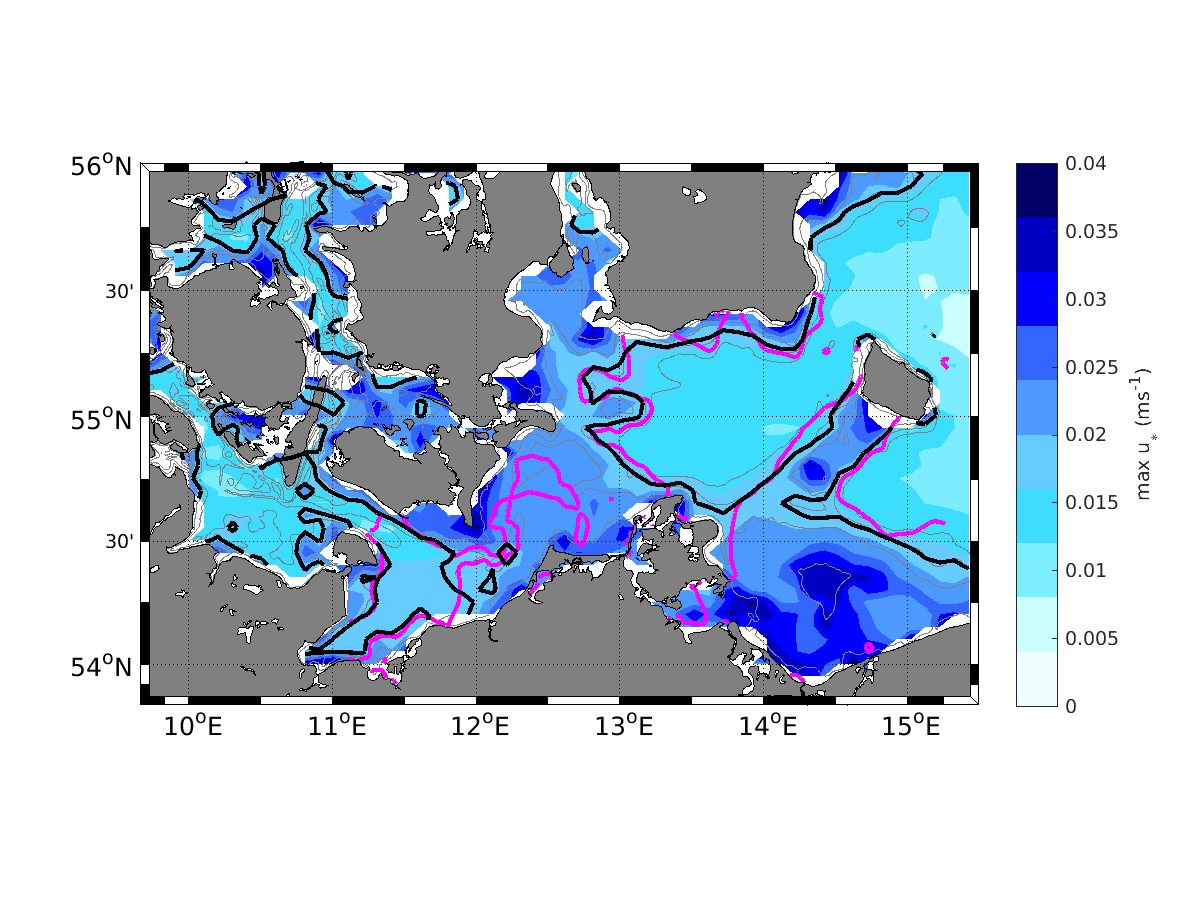
\includegraphics[width=16cm]{bilder/ubot_real.png}
 \caption{Calculated maximum $u_\ast$ using model outcome with realistic 
forcing from the year 2014. Gray lines show the 
isobaths at intervals of 10~m and the black line indicates $u_\ast = 0.02$ 
m~s$^{-1}$.\label{ustar_real}}
\end{figure}
\FloatBarrier
As visible in \fig{ustar_real}, high bottom friction velocities generally 
coincide with shallow water depth, but also topographic features, like 
sheltered bights or peninsulas, impact the effect of waves on the sea floor. 
The threshold of $u_\ast$ for resuspension of sediment depends on the present 
sediment type, sorting and biological factors (abundant species increase or 
decrease resuspension thresholds) and can therefore not be definitely determined 
from known parameters such as grain size distribution, although extrapolations 
exist. Most critical 
values for resuspension found in the literature range from $0.01$ to 
$0.03$~m~s$^{-1}$ \citep[][]{jonsson2004}. In \fig{ustar_real}, the black line 
indicates values of $u_\ast$ of $0.02$~m~s$^{-1}$ to give an orientation where 
waves play an important role for sediment dynamics.
% \section{Major Baltic Inflow December 2014}
% 
% In November 2014, medium to strong easterly winds forced an outflow of Baltic 
% sea water and consequently a drop in mean sea level of 57 cm. At the beginning 
% of December, the wind changed to heavily westerly wind, pushing a strong 
% barotropic inflow of saline water into the Baltic Sea. The main inflow period 
% lasted until Christmas. During that time, an overall amount of 320 $\text{km}^3$ 
% water was imported into the Baltic Sea, carrying approximately 4 Gt salt. The 
% MBI in 2014 was the third largest inflow event recorded since 1880 and has the 
% potential to ventilate the entire deep water of the Baltic. 
\FloatBarrier
\section{German Coastal Seas and Sediment}

General sedimentology and grain size distribution of parts of the Western 
Baltic Sea have 
been mapped in detail in a collaboration between the German maritime and 
hydrographic agency (BSH) and the Leibniz Institute for Baltic Sea Research 
(\fig{westernbaltic}). Prevailing sediments in this area reach from 
fine sand to silt. Although the sediment distribution is rather inhomogeneous, 
some 
features related to the bathymetry are clearly visible. In the very shallow 
regions with water depth less than 20 m, predominately sandy sediments are 
found, while in the deeper basins finer silt is present.
As fine grained material is easily eroded, it is not likely to remain in highly 
energetic, shallow regions and is therefore transported into the deeper basins, 
where 
it accumulates \citep[][]{basys1}. This process is best visible at the 
transition from the Oder Bight to the Arkona basin (see \fig{westernbaltic}b). 
It was found that the 20 m isobath separates erosional from depositional areas, 
and the muddy sediments accumulate below a regional halocline here 
\citep[][]{basys2}. The Arkona basin and surrounding area will be studied in 
more detail in the next section.

\begin{figure}[ht]
 \flushleft
 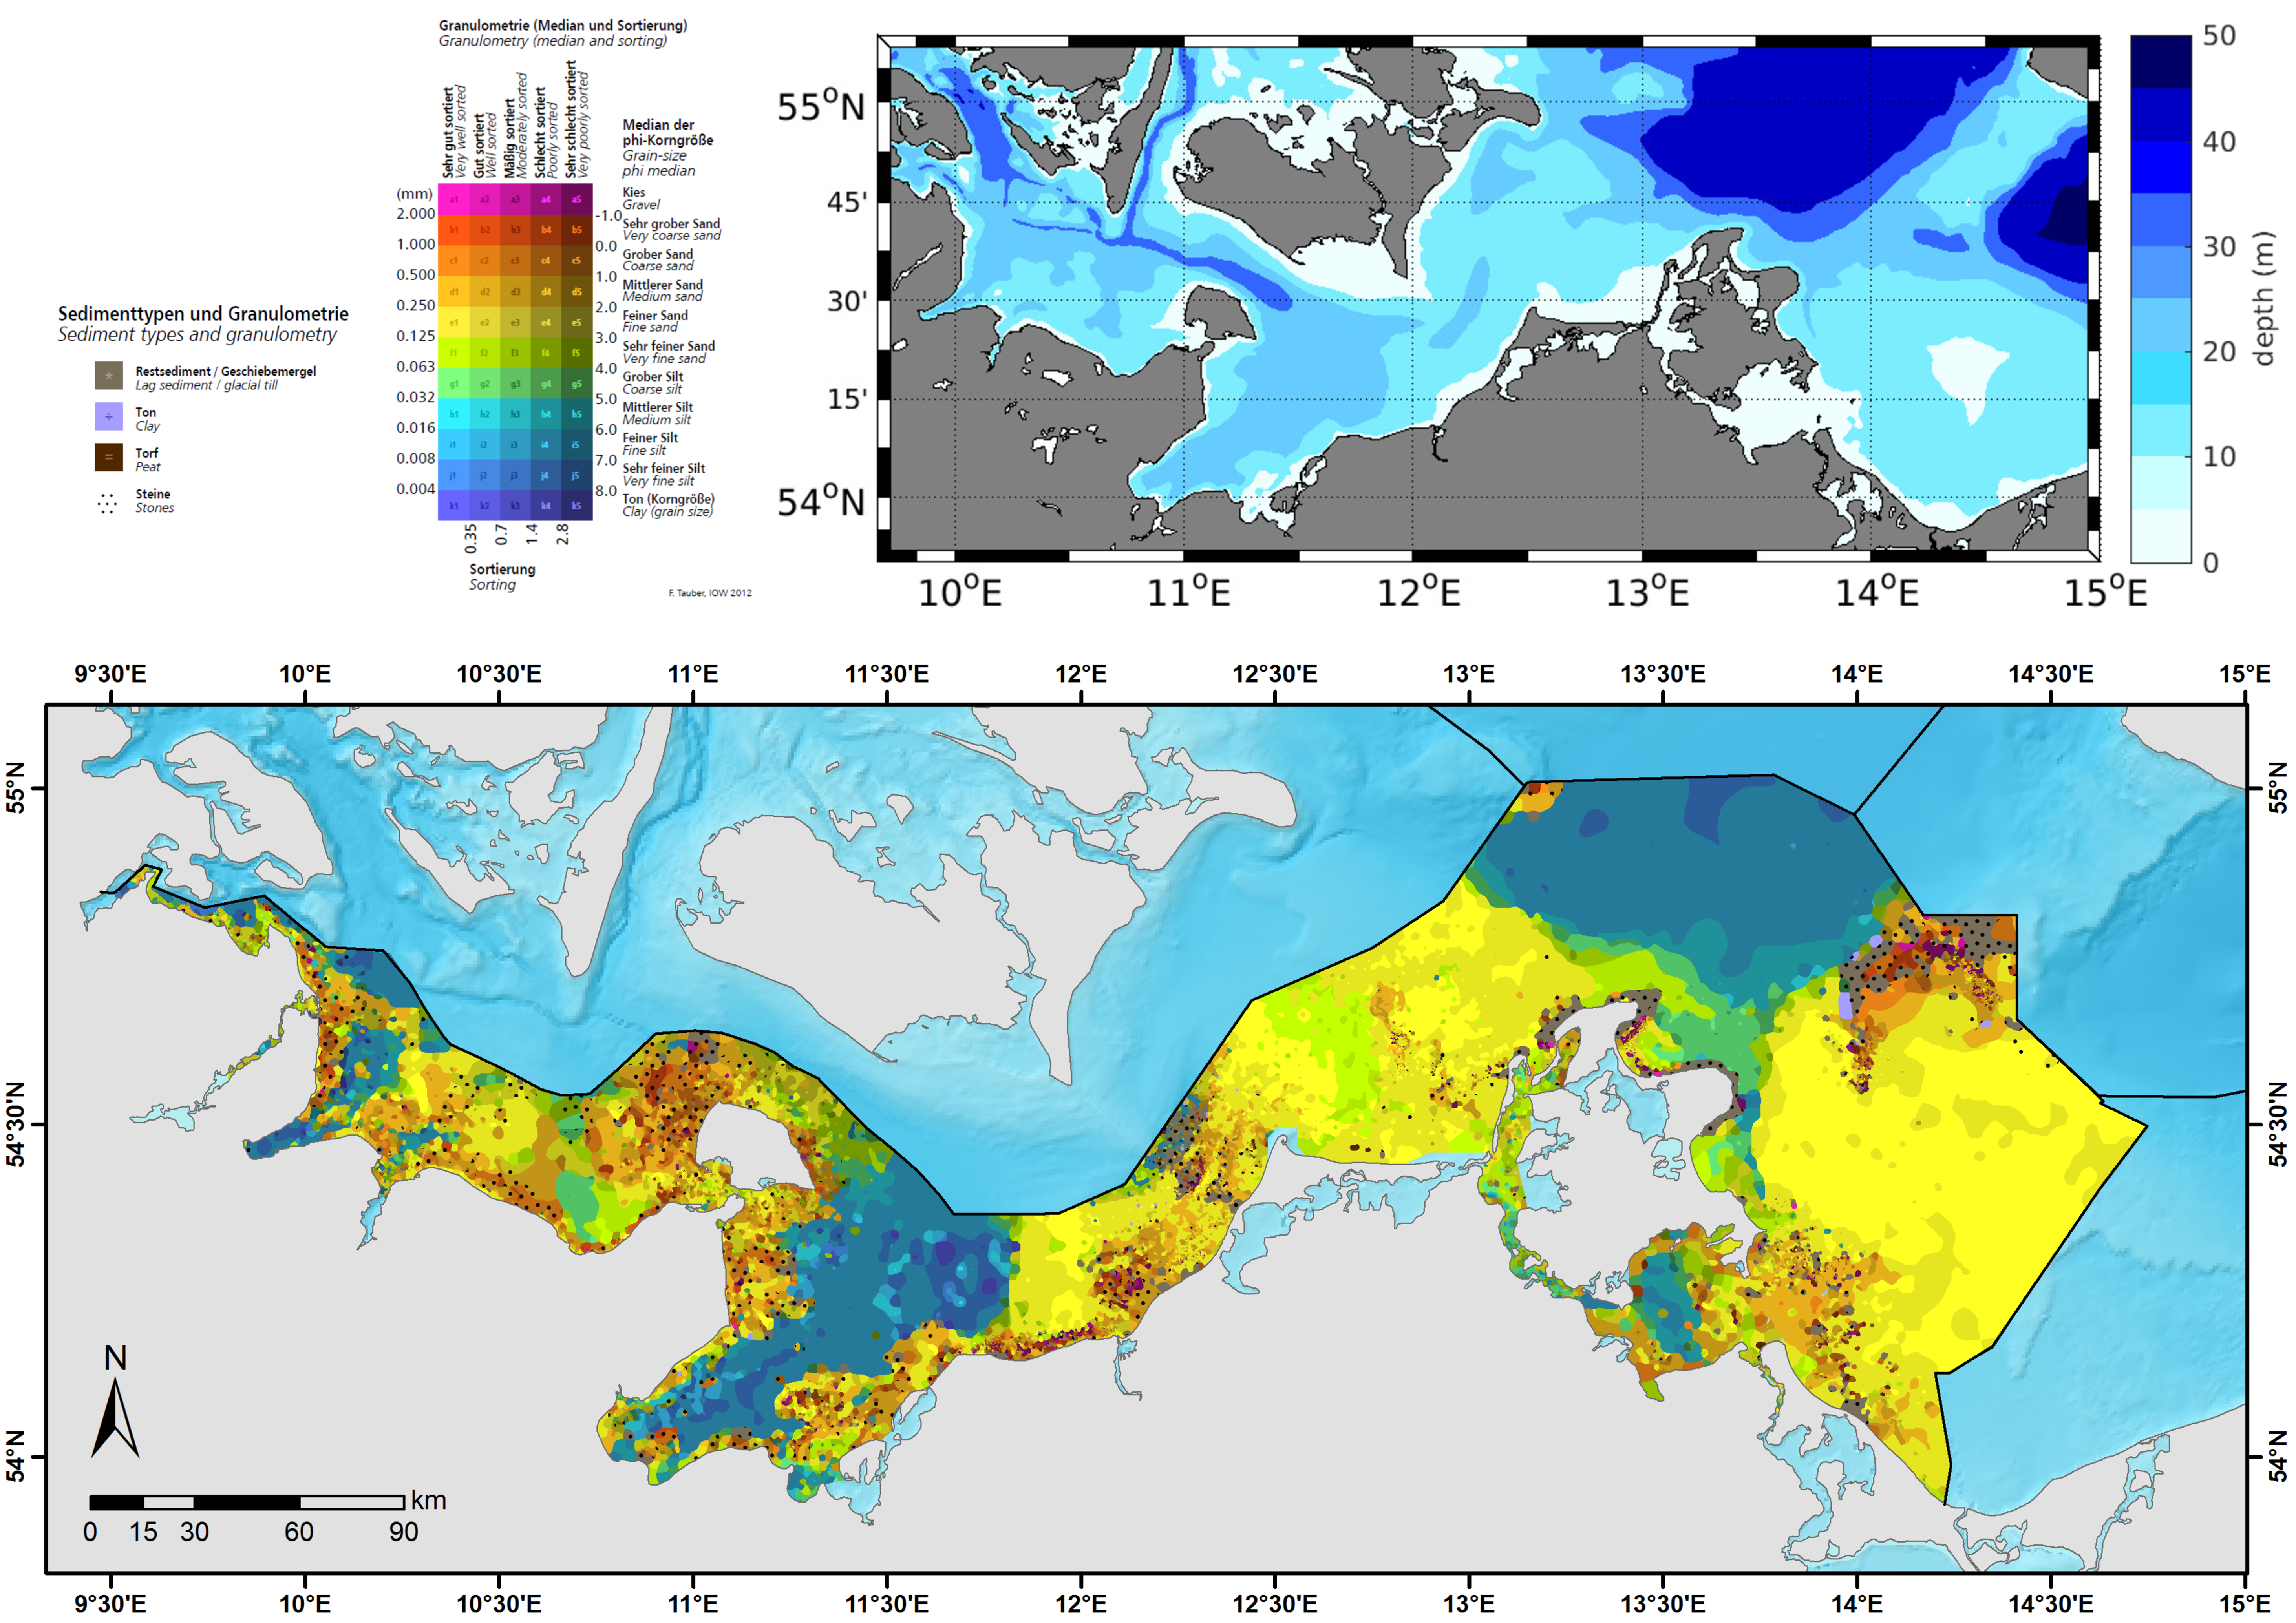
\includegraphics[width=16cm]{bilder/sediment.pdf}
 \caption{(a) Sediment and (b) topographic map of the Western Baltic 
Sea. Sediment data taken from \citep[][]{tauber2012}.}\label{westernbaltic}
\end{figure}